% Diagram figures (1, 2, 10) for the salience-weighted memory retrieval paper.
% Self-contained, compilable: pdflatex diagrams.tex  ->  diagrams.pdf
% Each figure is on its own page; crop to PDF/PNG per-figure for inclusion.
%
% These are the three schematic figures that are not auto-generated from data
% (the data figures 3-9 are SVGs in this directory). All labels/numbers trace to
% the technical report and FIGURE_PLAN.md.

\documentclass[tikz,border=8pt]{standalone}
\usepackage{tikz}
\usepackage{amsmath}
\usetikzlibrary{arrows.meta,positioning,fit,backgrounds,calc}
\usepackage{helvet}
\renewcommand{\familydefault}{\sfdefault}

\tikzset{
  sys/.style   ={rounded corners, draw, thick, align=center, minimum height=12mm,
                 minimum width=30mm, fill=blue!6},
  ghost/.style ={rounded corners, draw, dashed, align=center, minimum height=12mm,
                 minimum width=30mm, fill=black!4, text=black!55},
  stage/.style ={rounded corners, draw, thick, align=center, minimum height=11mm,
                 minimum width=26mm, fill=blue!6},
  pool/.style  ={draw, thick, align=center, minimum height=11mm, minimum width=26mm,
                 fill=orange!10},
  metric/.style={rounded corners, draw, thick, align=center, minimum height=11mm,
                 minimum width=26mm, fill=green!8},
  flow/.style  ={-{Stealth[length=3mm]}, thick},
  lbl/.style   ={font=\footnotesize, text=black!60},
  note/.style  ={font=\scriptsize\itshape, text=black!55},
}

\begin{document}

% =====================================================================
% Figure 1 — System Architecture
% =====================================================================
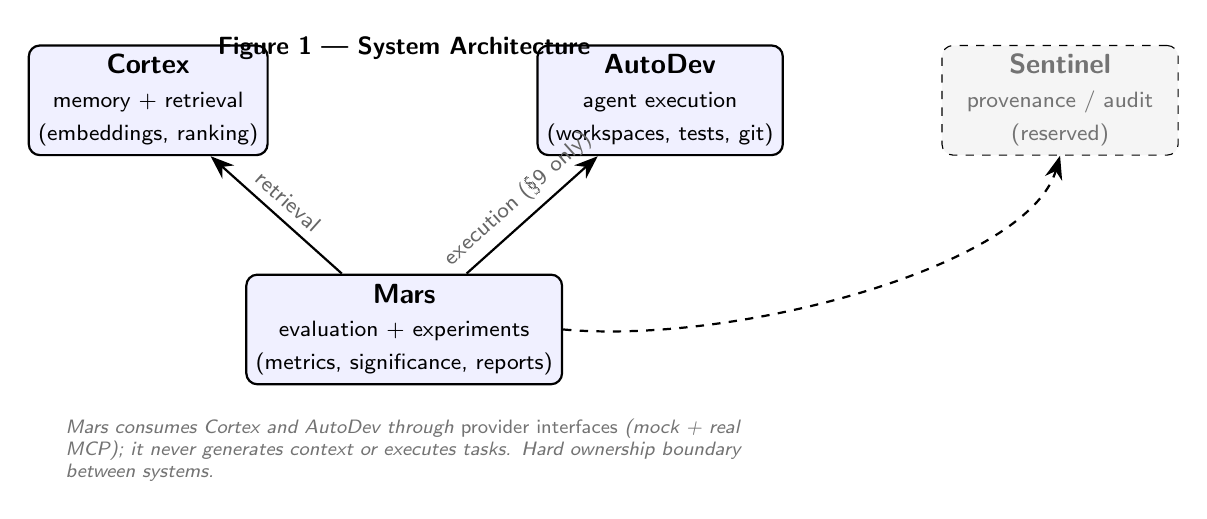
\begin{tikzpicture}[node distance=14mm]
  \node[sys]   (cortex) {\textbf{Cortex}\\\footnotesize memory + retrieval\\\footnotesize (embeddings, ranking)};
  \node[sys, right=34mm of cortex] (autodev) {\textbf{AutoDev}\\\footnotesize agent execution\\\footnotesize (workspaces, tests, git)};
  \node[sys, below=22mm of $(cortex)!0.5!(autodev)$] (mars) {\textbf{Mars}\\\footnotesize evaluation + experiments\\\footnotesize (metrics, significance, reports)};
  \node[ghost, right=20mm of autodev] (sentinel) {\textbf{Sentinel}\\\footnotesize provenance / audit\\\footnotesize (reserved)};

  \draw[flow] (mars) -- node[lbl, sloped, above]{retrieval} (cortex);
  \draw[flow] (mars) -- node[lbl, sloped, above]{execution (\S9 only)} (autodev);
  \draw[flow, dashed] (mars.east) .. controls +(2.2,-0.2) and +(-0.4,-1.4) .. (sentinel.south);

  \node[note, below=3mm of mars, text width=86mm]
    {Mars consumes Cortex and AutoDev through \emph{provider interfaces}
     (mock + real MCP); it never generates context or executes tasks.
     Hard ownership boundary between systems.};
  \node[font=\small\bfseries, above=4mm of $(cortex)!0.5!(autodev)$] {Figure 1 — System Architecture};
\end{tikzpicture}

% =====================================================================
% Figure 2 — Retrieval Pipeline
% =====================================================================
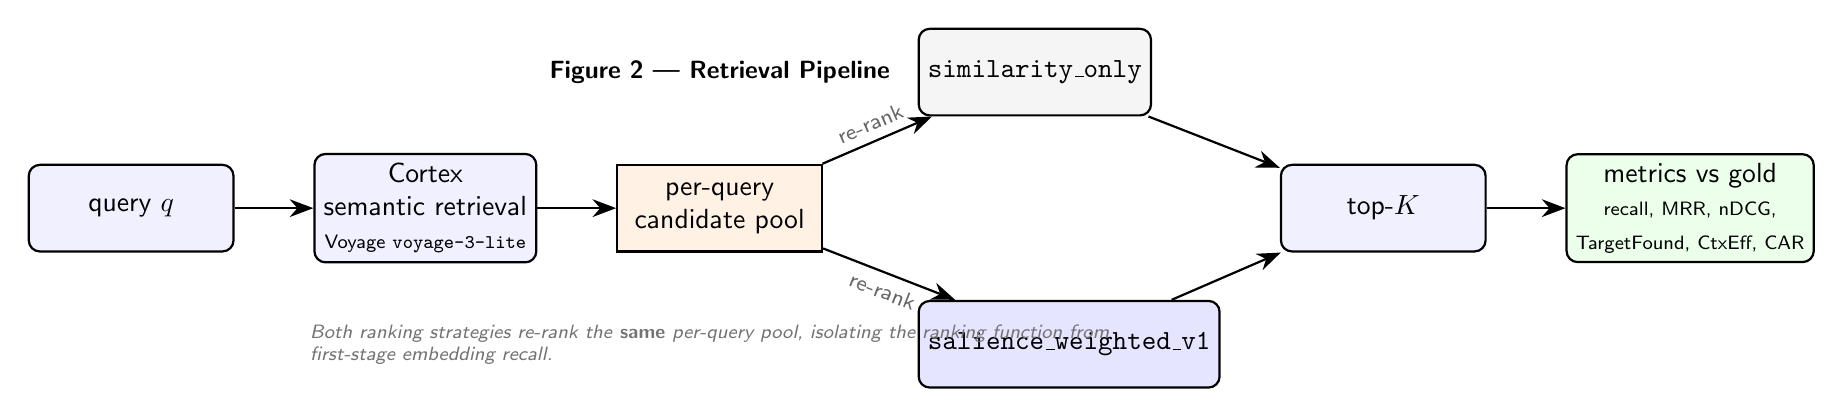
\begin{tikzpicture}[node distance=10mm]
  \node[stage] (q) {query $q$};
  \node[stage, right=10mm of q] (ret) {Cortex\\semantic retrieval\\\scriptsize Voyage \texttt{voyage-3-lite}};
  \node[pool,  right=10mm of ret] (pool) {per-query\\candidate pool};
  \node[stage, above right=6mm and 12mm of pool, fill=black!4] (a) {\texttt{similarity\_only}};
  \node[stage, below right=6mm and 12mm of pool, fill=blue!10] (b) {\texttt{salience\_weighted\_v1}};
  \node[stage, right=58mm of pool] (topk) {top-$K$};
  \node[metric, right=10mm of topk] (m) {metrics vs gold\\\scriptsize recall, MRR, nDCG,\\\scriptsize TargetFound, CtxEff, CAR};

  \draw[flow] (q) -- (ret);
  \draw[flow] (ret) -- (pool);
  \draw[flow] (pool) -- node[lbl,sloped,above]{re-rank} (a);
  \draw[flow] (pool) -- node[lbl,sloped,below]{re-rank} (b);
  \draw[flow] (a) -- (topk);
  \draw[flow] (b) -- (topk);
  \draw[flow] (topk) -- (m);

  \node[note, below=8mm of pool, text width=104mm]
    {Both ranking strategies re-rank the \textbf{same} per-query pool, isolating the
     ranking function from first-stage embedding recall.};
  \node[font=\small\bfseries, above=9mm of pool] {Figure 2 — Retrieval Pipeline};
\end{tikzpicture}

% =====================================================================
% Figure 10 — Research Program Overview
% =====================================================================
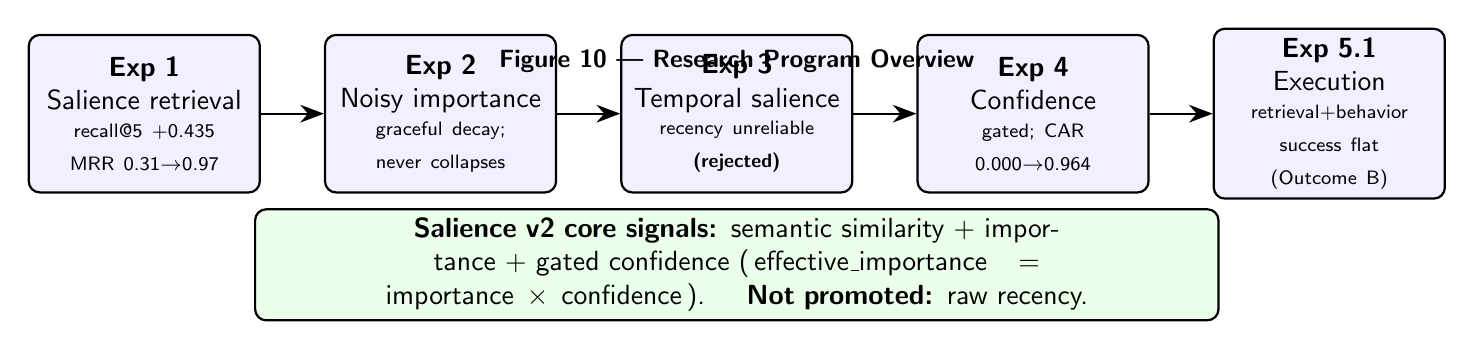
\begin{tikzpicture}[node distance=6mm]
  \tikzset{exp/.style={rounded corners, draw, thick, align=center,
           minimum height=20mm, text width=27mm, fill=blue!6}}
  \node[exp] (e1) {\textbf{Exp 1}\\Salience retrieval\\[2pt]\scriptsize recall@5 +0.435\\\scriptsize MRR 0.31$\to$0.97};
  \node[exp, right=8mm of e1] (e2) {\textbf{Exp 2}\\Noisy importance\\[2pt]\scriptsize graceful decay;\\\scriptsize never collapses};
  \node[exp, right=8mm of e2] (e3) {\textbf{Exp 3}\\Temporal salience\\[2pt]\scriptsize recency unreliable\\\scriptsize \textbf{(rejected)}};
  \node[exp, right=8mm of e3] (e4) {\textbf{Exp 4}\\Confidence\\[2pt]\scriptsize gated; CAR\\\scriptsize 0.000$\to$0.964};
  \node[exp, right=8mm of e4] (e5) {\textbf{Exp 5.1}\\Execution\\[2pt]\scriptsize retrieval+behavior\\\scriptsize success flat (Outcome B)};

  \foreach \a/\b in {e1/e2, e2/e3, e3/e4, e4/e5}
    \draw[flow] (\a) -- (\b);

  \node[rounded corners, draw, thick, fill=green!8, align=center,
        below=12mm of $(e2)!0.5!(e4)$, text width=120mm] (panel)
    {\textbf{Salience v2 core signals:} semantic similarity $+$ importance $+$ gated
     confidence (\,$\text{effective\_importance}=\text{importance}\times\text{confidence}$\,).
     \quad \textbf{Not promoted:} raw recency.};

  \node[font=\small\bfseries, above=4mm of $(e1)!0.5!(e5)$] {Figure 10 — Research Program Overview};
\end{tikzpicture}

\end{document}
